\documentclass[Japanese]{dicomopapers}
%\documentclass[Japanese,noauthor]{dicomopapers}

% \usepackage[dvips]{graphicx}
\usepackage{latexsym}
\usepackage[dvipdfmx]{graphicx}

\usepackage[utf8]{inputenc}
\usepackage{array}
\usepackage{amssymb} % 数学記号用
\usepackage{scalefnt}
\usepackage{makecell}
\usepackage{float}
\usepackage{booktabs} 
\usepackage{listings}

\providecommand{\newblock}{}





\def\Underline{\setbox0\hbox\bgroup\let\\\endUnderline}
\def\endUnderline{\vphantom{y}\egroup\smash{\underline{\box0}}\\}
\def\|{\verb|}

\usepackage{caption}
\lstset{
  basicstyle={\ttfamily},
  identifierstyle={\small},
  commentstyle={\smallitshape},
  keywordstyle={\small\bfseries},
  ndkeywordstyle={\small},
  stringstyle={\small\ttfamily},
  frame={tb},
  breaklines=true,
  columns=[l]{fullflexible},
  numbers=left,
  xrightmargin=0zw,
  xleftmargin=3zw,
  numberstyle={\scriptsize},
  stepnumber=1,
  numbersep=1zw,
  lineskip=-0.5ex
}


\begin{document}

% 和文表題
\title{様々な状況と環境に対応できる\\PDRベースの屋内位置推定ライブラリの基礎検討}
% 英文表題
\etitle{
	Consideration of a PDR-based indoor location estimation library for various situations and environments}

% 所属ラベルの定義
\affiliate{IPSJ}{(社)情報処理学会\\
	IPSJ}
\paffiliate{DICOMO}{マルチメディア,分散,協調とモバイルシンポジウム\\DICOMO2023}

\author{外山 瑠起}{TOYAMA RYUKI}{IPSJ}
\author{梶 克彦}{KAZI KATSUHIKO}{DICOMO}

\begin{abstract}
	現代の社会において,屋内位置推定技術は重要な技術である.
	屋内の人の動きを把握してビル内のナビゲーションなどに活用するなど様々な活用方法が考えられる.
	しかし,屋内での位置推定は外部環境に大きく影響され,使用できるデータが異なるため,特定の屋内位置推定手法であらゆる場面に対応するのは困難である.
	多様な状況や環境で屋内位置推定をするには,個々の条件に適した位置推定手法の組み合わせや選択が重要である.
	例として歩行者の初期位置とスマートフォンから加速度,角速度,設置されたBLEビーコンからの電波強度が使用できる場合.PDRに加えてBLEの電波強度をしてPDRによる誤差を補正できる.
	このように状況に応じて適切な処理を行えば,より精度のよい屋内位置推定が可能になる.
	本研究の目的は様々な状況と環境に柔軟に対応できる,包括的な屋内位置推定ライブラリの開発である.
\end{abstract}

% 表題などの出力
\maketitle

% 本文はここから始まる
\section{はじめに}
屋内位置置推定技術は,現代社会において重要な役割を果たしており様々な活用が期待できる.
屋内位置推定技術が使用される一例として,ショッピングモール施設でのナビゲーションシステムが挙げられる[1].
このシステムでは顧客が店内で商品を探している際,その位置情報を元にしたナビゲーションシステムを通じて目的の商品が置かれている売り場まで案内するシステムである.

屋外における位置推定技術としてGPSが広く利用されているが,屋内環境では建物の壁や天井がGPS衛星からの電波を遮断してしまい,位置推定精度が大きく低下してしまう問題があり,別のアプローチが必要とされている.
屋内位置推定手法として,PDR(Pedestrian Dead Reckoning)が挙げられる.
PDRは主に,加速度計,ジャイロスコープ,磁気センサなどのセンサを利用して歩行者のステップ数,歩行速度,歩行方向を推定する.
その情報を元に歩行者がどのくらいの距離をどの方向に移動したかを累積的に計算して基準となる位置からの相対的な位置を推定する手法である.
他の例として,Wi-Fiの電波を使用した屋内位置推定手法がある.
Wi-Fiを利用した屋内位置推定は,Wi-Fiアクセスポイントからの信号強度を利用して位置推定を行う.特定の地点でのフィンガープリントを予め取得しておきそれと比較して推定を行う手法や,3つのアクセスポイントからの電波強度を利用して三角測量を行う手法がなどがある.

しかしこれらの手法は特定の状況や環境に特化したものであり,すべての屋内環境で同様の効果を発揮するわけではない.例として先ほどあげたWi-Fiを利用した屋内位置推定の場合,地下施設やWi-Fiアクセスポイントが設置が難しい場所では,信号が弱いため正確な位置推定が難しくなる.
PDRの場合各種センサによる誤差が蓄積されるため,時間経過とともに誤差が大きくなってしまう問題がある.そのため長時間の屋内移動場合は精度が低下してしまう.

これらの問題を解決するためには状況や環境に応じて適切な位置推定手法の選択または組みわせる必要がある.
本研究の目的は様々な環境に対応できるオフライン屋内位置推定ライブラリの検討である.
ここでいうオフラインとは,あらかじめ取得したデータを元に位置推定を行うという意味である.
先ほどあげた長時間の屋内移動の場合,PDRで推定した位置情報をWi-Fiの電波強度を利用した位置推定でセンサの誤差を修正すれば,より正解な位置推定を行える.
これらの補正を自由に組み合わせて使えるライブラリの検討を行い,様々な状況に対応できるオフライン屋内位置推定ライブラリを実現する.

\section{関連研究}
屋内位置推定の手法において環境内に設置された機器を利用し推定する絶対位置測位手法がある.
絶対位置測位は,屋内に設置された機器からの情報を元に位置を推定する手法である.
例えばBluetoothやWi-Fiなどの電波を利用した手法がある.
屋内に設置した近接特化型のBLEビーコン3つからの電波強度を利用して三角測量を行い位置推定を行う研究\cite{ble-indoor}や
GMMを使用してWi-Fiの電波強度分布をモデル化し,それを元に位置推定を行う研究\cite{wifi-gmm}がある.
これらの手法は設置された機器がない場合や設置が難しい場合は使用できない問題がある.

PDRと絶対位置測位を組み合わせて屋内位置推定を行う手法がある.
PDRとWi-Fiの受信強度を用いたプロキシミティベースの位置推定を行う研究\cite{pdr-wifi}やBLEビーコンの受信信号強度の変異を
利用した移動変異推定とPDRとの併用による累積測位誤差の補正を行う研究\cite{pdr-ble}がある.
またPDRとマップマッチングを組み合わせて位置推定を行う研究\cite{pdr-map}や
歩行時の磁気データのみを用いて位置推定を行う研究\cite{pdr-mag}がある.
これらの研究で示されているようにPDRと絶対位置測位を組み合わせた手法は,
お互いのデメリットを補えるため屋内位置推定をする上で有用な手法である.

本研究でもPDRによる位置推定を行いその結果に対して,BLEビーコンの電波強度を使用した補正やマップマッチングによる
補正をなどが行えるライブラリを検討する.
さらに初期位置や終了位置などの様々な状況の情報で補正できるように
より包括的かつ柔軟な屋内位置推定ライブラリの検討を行う.
\section{PDRベースの屋内位置推定ライブラリの検討}

\subsection{要求仕様}

屋内位置推定は状況や環境によって推定に使用できる情報が異なるため,
ライブラリを作る上でその具体的な例を考える必要がある.
例えば,大学内や病院などのWi-Fiのアクセスポイントが多く設置されている場所では
Wi-Fiの電波強度を利用した位置推定が有効である.
他の例として展示会場や大きなアトリウムなどの広い開放空間が考えられる.
このような場所ではWi-Fiのアクセスポイントの配置が難しく,信号のカバレッジが不均一
になりやすくWi-Fiを利用した位置推定は難しい.
このような場所の場合BLEビーコンを配置してその電波強度を利用した位置推定ができると考えられる.
正しこのような空間で正確な位置推定を行うには,BLEビーコンの多数配置する必要があり,
労力や配置したとしてもメンテナンスコストがかかる可能性がある.
このような場合はPDRを利用した位置推定が有効である.
PDRは歩行者の歩行速度や歩行方向を推定して位置推定を行う手法である.
この手法では歩行者がスマートフォンを持っているだけで良いため,先ほどあげたような
場所でもコストをかけずに位置推定を行えると考えられる.
しかしPDRはセンサのわずかな誤差が,時間経過とともに蓄積され位置推定の誤差が大きくなってしまう問題がある.
そのため長時間の歩行の場合は位置推定の精度が低下してしまう.
このような問題を解決する手法として\cite{pdr-wifi}や\cite{pdr-ble}や方法が提案されている.

これらの手法のように基本的なベースをPDRで位置推定を行い,その結果を補正できるようなライブラリの検討を行う.
ライブラリを作る上での想定環境としてXDR Challenge Track5の環境を元に考える.
XDR Challengeは屋内位置推定の精度を競うコンテストである.
このコンテストのTrack5では歩行者が高速道路のサービスエリアを歩行する.
歩行者は腰にスマートフォンをつけた状態でLiDARと呼ばれる光を使った距離測定技術を搭載した
ハンドヘルドLiDAR(以下,LiDAR)を持ち施設内を歩行する.
参加者にはスマートフォンから得られた,加速度,角速度,磁気センサのデータとLiDARから
得られた正解の歩行軌跡の座標が提供される.
施設内にはBLEビーコンが配置されており,歩行時の各ビーコンからの電波受信強度が提供される.
他に与えられるデータとして,フロアマップ情報,フロアマップにおける各BLEビーコンの配置情報,
歩行者の初期位置,終了位置が与えられる.
本来であれば病院や学校などのより多くの施設で利用できるライブラリにする必要がある.
しかしそのようなライブラリを構築するのは難しいためまず基本的な屋内位置推定環境が整っている
XDR Challngeの環境でのライブラリの基礎検討と検証を行う.


関数に必要な引数の情報とその対応表を表1に示す.
詳しい関数の説明や内部実装については次節で述べる.
引数の情報は大きく分けてセンサ情報,環境情報,その他の3つに分けられる.
センサ情報はスマートフォンから得られる加速度,角速度,磁気センサ,BLEビーコンの電波情報が含まれる.
環境情報はフロアマップ情報,フロアマップにおける各BLEビーコンの配置情報が含まれる.
これらの環境情報は全てセンサデータが与えられる前に得られる情報である.
その他はセンシング中,またはセンシング前に得られる情報であり,初期位置,終了位置などの情報が該当する.

\subsection{ライブラリ}
\begin{table*}[ht]
	\centering
	\scalebox{0.7}{
		\begin{tabular}{|c|c|c|c|c|c|c|c|c|c|c|c|} % Change 'l' to 'c' for center alignment
			\hline
			              & \multicolumn{3}{c|}{センサ情報}   & \multicolumn{4}{c|}{環境情報}    & \multicolumn{4}{c|}{その他}                                                                                                                                                                                                                                                                    \\ \hline
			              &                              &                              & \multicolumn{1}{c|}{BLEビーコン} &        & \makecell{磁気                                                                                                } & \multicolumn{2}{c|}{BLEビーコン} & \multicolumn{2}{c|}{正解初期}    & \multicolumn{2}{c|}{補正}                                               \\ \cline{4-4} \cline{6-6} \cline{7-7} \cline{8-8}\cline{9-10}\cline{11-12}
			              & 加速度                          & 角速度                          & 電波強度                         & フロアマップ & FP                                                                                                            & 基地局位置                        & FP                           & 座標                           & 方向 & 座標                           & 方向 \\ \hline
			基本PDR         & \multicolumn{1}{c|}{$\circ$} & \multicolumn{1}{c|}{$\circ$} &                              &        &                                                                                                               &                              &                              &                              &    &                              &    \\ \hline
			正解初期座標が存在     & \multicolumn{1}{c|}{$\circ$} & \multicolumn{1}{c|}{$\circ$} &                              &        &                                                                                                               &                              &                              & \multicolumn{1}{c|}{$\circ$} &    &                              &    \\ \hline
			ドリフト補正        & \multicolumn{1}{c|}{$\circ$} & \multicolumn{1}{c|}{$\circ$} &                              &        &                                                                                                               &                              &                              & \multicolumn{1}{c|}{$\circ$} &    & \multicolumn{1}{c|}{$\circ$} &    \\ \hline
			初期方向補正 フロアマップ & \multicolumn{1}{c|}{$\circ$} & \multicolumn{1}{c|}{$\circ$} &                              &        & \multicolumn{1}{c|}{$\circ$}                                                                                  &                              &                              &                              &    &                              &    \\ \hline
			初期方向補正 BLE    & \multicolumn{1}{c|}{$\circ$} & \multicolumn{1}{c|}{$\circ$} & \multicolumn{1}{c|}{$\circ$} &        &                                                                                                               & \multicolumn{1}{c|}{$\circ$} &                              &                              &    &                              &    \\ \hline
			マップマッチング補正    & \multicolumn{1}{c|}{$\circ$} & \multicolumn{1}{c|}{$\circ$} &                              &        & \multicolumn{1}{c|}{$\circ$}                                                                                  &                              &                              &                              &    &                              &    \\ \hline
			安定歩行区間補正      & \multicolumn{1}{c|}{$\circ$} & \multicolumn{1}{c|}{$\circ$} &                              &        &                                                                                                               &                              &                              &                              &    &                              &    \\ \hline
			初期方向補正 BLE FP & \multicolumn{1}{c|}{$\circ$} & \multicolumn{1}{c|}{$\circ$} &                              &        &                                                                                                               &                              & \multicolumn{1}{c|}{$\circ$} &                              &    &                              &    \\ \hline
		\end{tabular}
	}
	\caption{関数に必要な情報とその対応表} \label{}
\end{table*}


\begin{table}[h]
	\centering
	\begin{tabular}{lll}
		\toprule
		カラム名 & 単位          & データ型      \\
		\midrule
		ts   & s (seconds) & timestamp \\
		x    & m/s\(^2\)   & float     \\
		y    & m/s\(^2\)   & float     \\
		z    & m/s\(^2\)   & float     \\
		\bottomrule
	\end{tabular}
	\caption{加速度 DF}
\end{table}

\begin{table}[h]
	\centering
	\begin{tabular}{lll}
		\toprule
		カラム名 & 単位             & データ型      \\
		\midrule
		ts   & s (秒)          & timestamp \\
		x    & rad/s (ラジアン/秒) & float     \\
		y    & rad/s (ラジアン/秒) & float     \\
		z    & rad/s (ラジアン/秒) & float     \\
		\bottomrule
	\end{tabular}
	\caption{角速度 DF}
\end{table}

\begin{table}[h]
	\centering
	\begin{tabular}{l l}
		\hline
		キー名 & データ型  \\
		\hline
		"x" & float \\
		"y" & float \\
		\hline
	\end{tabular}
	\caption{初期座標 DICT}
\end{table}

以下節で説明する関数の引数に必要な情報は全て表1と紐づいている.
まず基本的なPDRの処理を行う関数をリスト\ref{lst:hoge}に示す.
この関数では加速度(acc),角速度(gyro)を使用して位置推定を行う.
加速度,角速度のデータフレームのカラム名とデータ型を表2,表3に示す.
初期座標は辞書型で表4に示す.

歩幅の推定を行っている研究は多くある.
機会学習を用いた研究\cite{stride-length-auto-learning},
多変量解析を用いた研究\cite{stride-length-multi},
超音波センサーガジェットを用いた研究\cite{stride-length-ultrasonic}などがある.
本関数の内部処理では歩幅の値は固定値として扱っている.
本来であれば歩幅は身長,性別,年齢などの複数の要素によって動的に変化するため
固定値なのはありえず,先ほど挙げた研究のように歩幅を推定する必要がある.
しかし本ライブラリの目的は正確な歩幅を用いたPDRによる位置推定ではない.
PDRで推定した歩行軌跡を環境情報などを用いて補正を行い軌跡全体の最適化を行えるライブラリの検討である.
そのため歩幅の推定は行わず固定値として扱う.
また同様の理由で歩行タイミングの検出も正確には行わず,加速度の値が特定の閾値を超えた時に歩行タイミングとして扱っている.
図\ref{fig:pdr}にリスト\ref{lst:hoge}を用いてPDRによる位置推定を行った結果を示す.
LiDARで取得した座標をもとに出力された軌跡を図\ref{fig:gt-trajectory}に示しこれを本論では正解軌跡とする.
図1と図2を比較するとPDRによる軌跡は正解軌跡と比べて大きくずれているのがわかる.
PDR特有の解決すべき問題として,
軌跡そのものの形状を正解奇跡に近づける問題と絶対位置との関連付けに分けられる.


PDRによって出力された軌跡を環境情報などを用いて補正を行い正解軌跡に近づけていく.


\begin{lstlisting}[caption = {基本PDR}, label = {lst:pdr-trajectory}]
def estimate_trajectory(
    acc: pd.DataFrame,
    gyro: pd.DataFrame,
    first_point: dict,
) 
\end{lstlisting}

\begin{figure}[h]
	\centering
	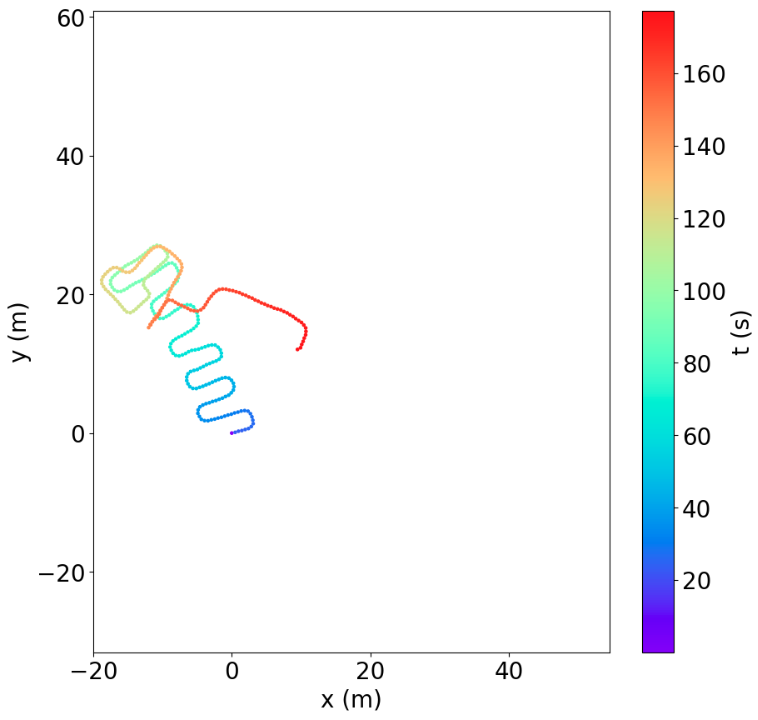
\includegraphics[width=80mm]{image/pdr.jpg}
	\caption{PDRによる軌跡}    \label{fig:pdr}
\end{figure}

正解初期座標が予め判明している場合にリスト\ref{lst:pdr-trajectory}に示される関数に
その座標を与えたのが図\ref{fig:pdr-move}である.

\begin{figure}[h]
	\centering
	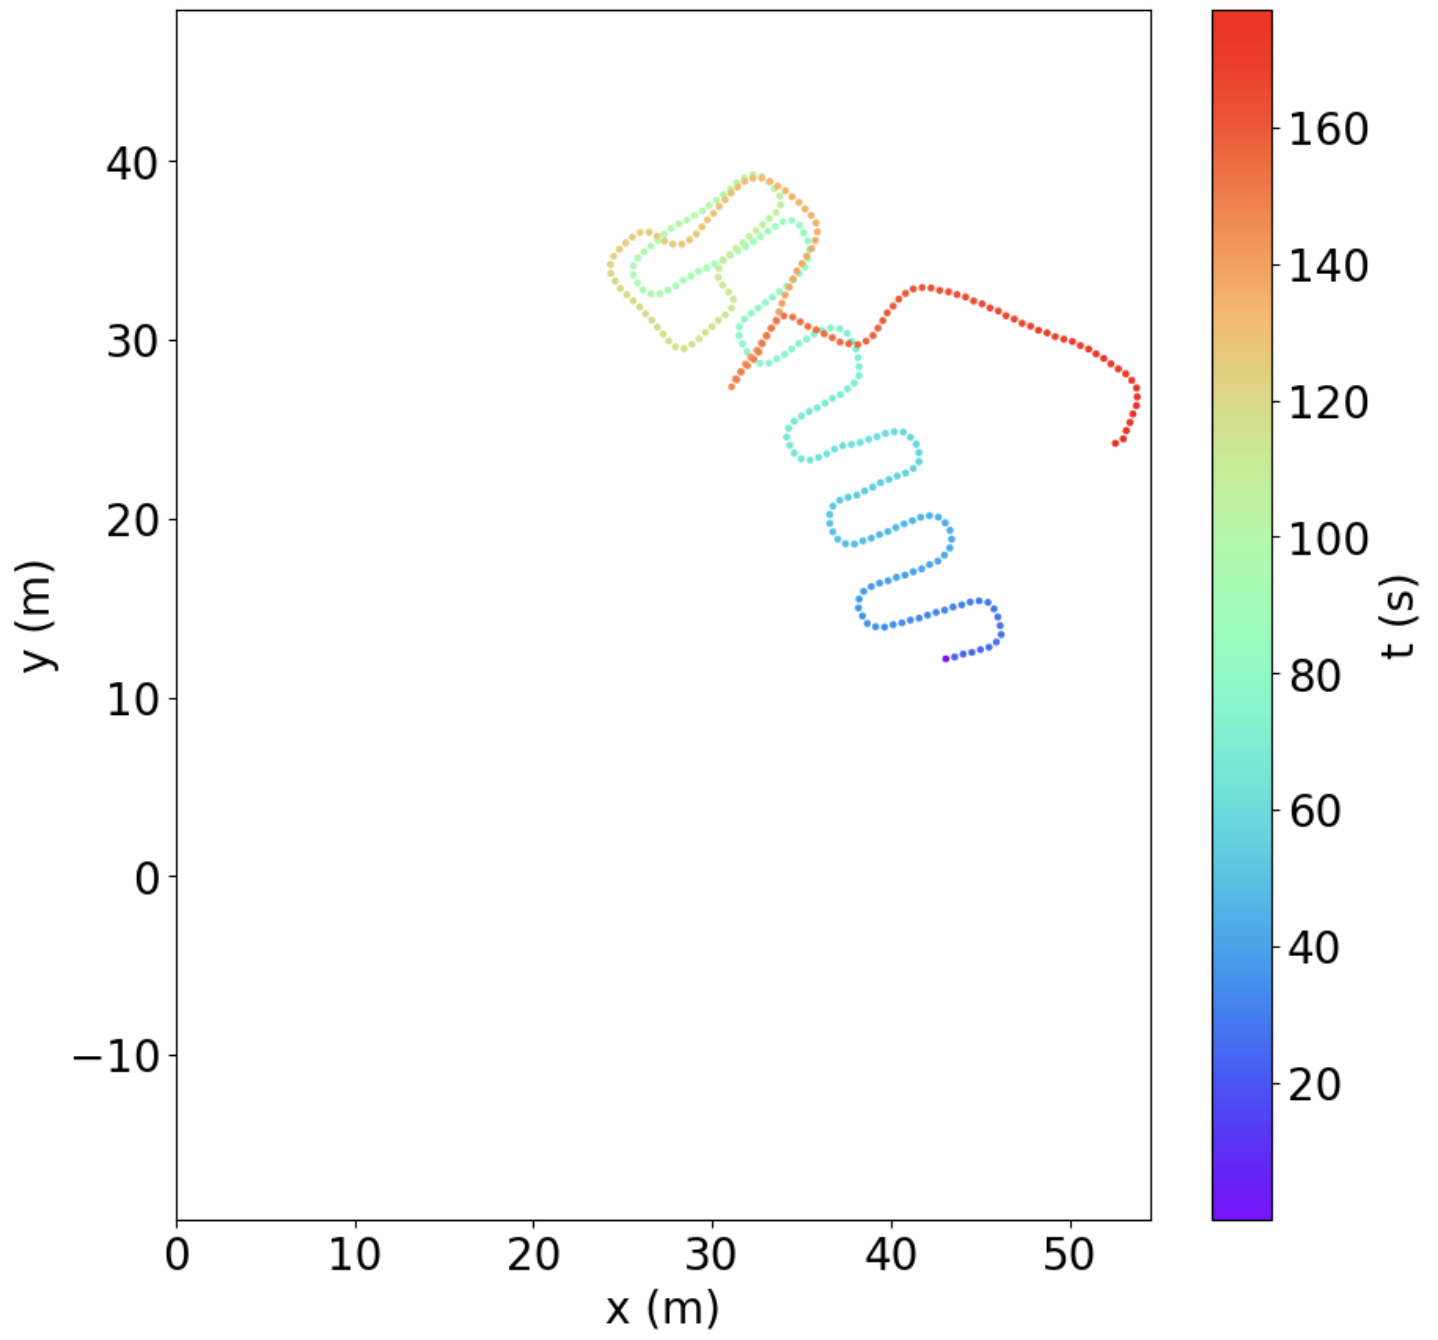
\includegraphics[width=80mm]{image/pdr-move.jpg}
	\caption{正解初期座標が存在}    \label{fig:pdr-move}
\end{figure}

\begin{figure}[h]
	\centering
	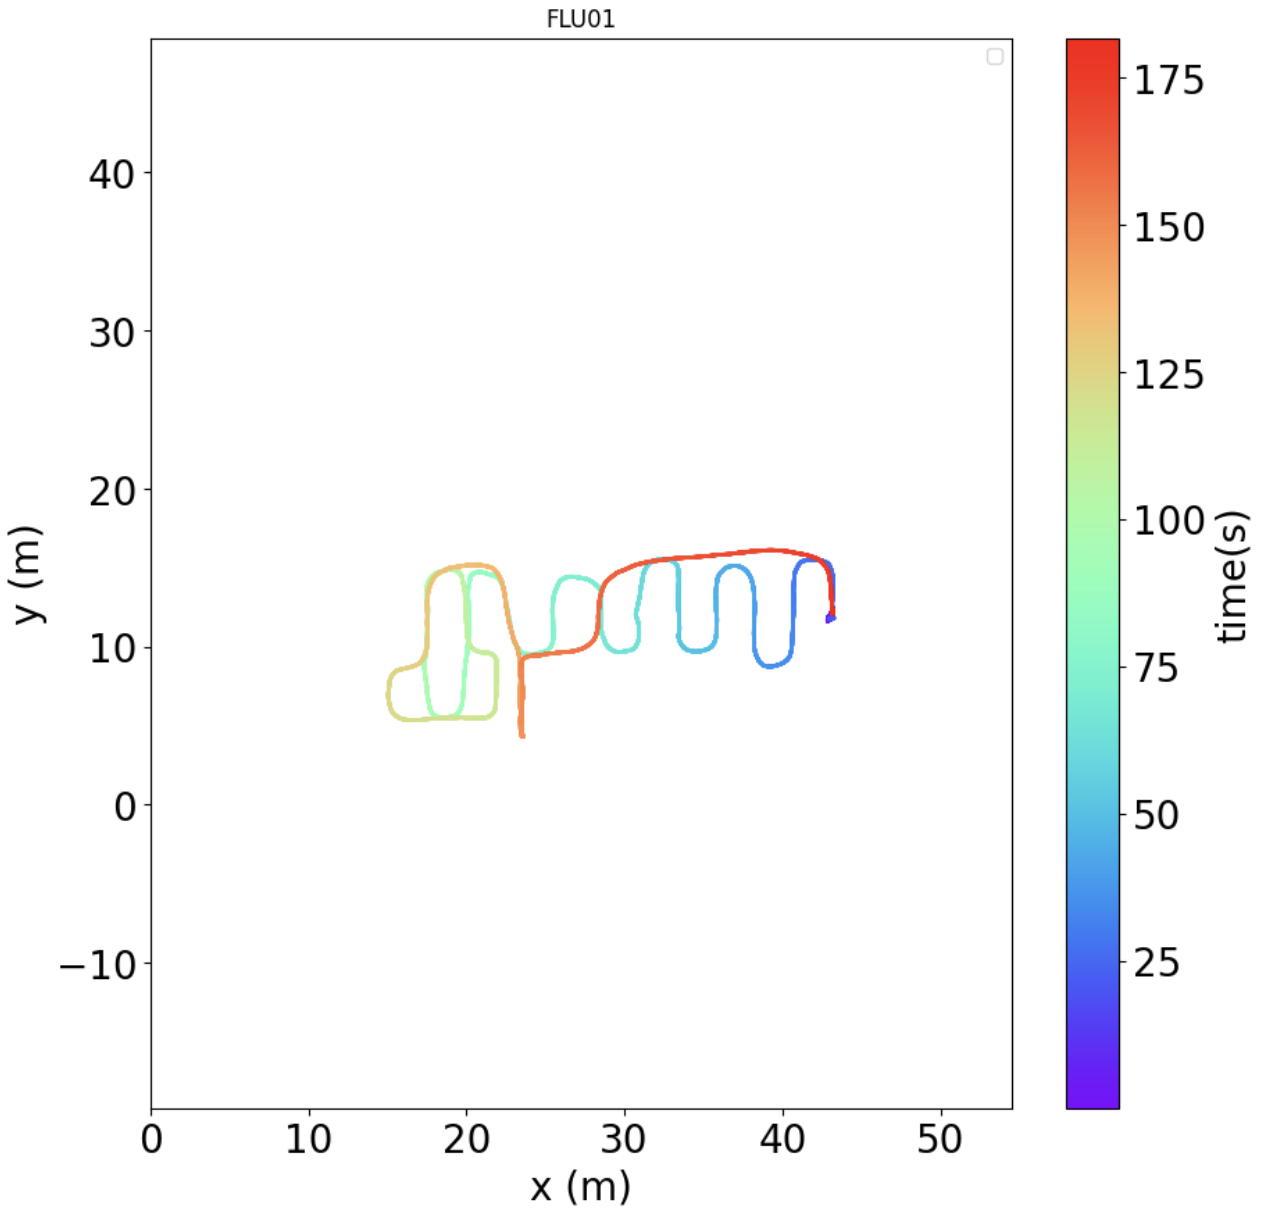
\includegraphics[width=80mm]{image/gt2.jpg}
	\caption{正解軌跡}    \label{fig:gt-trajectory}
\end{figure}


図\ref{fig:pdr-move}の軌跡にはPDR特有のドリフト現象が見られる.
PDRでは角速度から進行方向を求めてその方向を元に歩行軌跡を描く.
そのため角速度センサーにわずかなでも誤差が含まれると時間経過とともにその誤差が大きくなり軌跡の形状が本来の軌跡から外れる.
この問題を解決するために,角速度データに含まれる累積誤差を取り除く必要がある.
我々は特定のアルゴリズムを導入した.
% このアルゴリズムは,角速度データに含まれる累積誤差を取り除くことで,PDRに基づく軌跡の精度を向上させる。
ドリフト補正のプロセスは,ドリフトを動的に計算し,それを角度データから差し引くことで補正を行う.具体的には、
`apply\_remove\_drift\_to\_angle`関数を用いて,各時点での角度データからドリフトを除去する。
この関数は,角度データフレーム,ドリフトの値,引数として取り、補正された角度データフレームを返す.
このドリフト補正プロセスは,式(1)で表される.
$\theta'(t)$は時間$t$における補正後の角度,$\theta(t)$は補正前の角度,
$\mathrm{d}$はドリフト率を意味する.
この式は,時間経過に伴うドリフトの累積効果を補正するために使用される.

\vspace{5mm} % 5mmの空白を追加。必要に応じて値を調整してください。

\begin{equation}
	\theta'(t) = \theta(t) - (\mathrm{d} \times (t))
\end{equation}

\vspace{5mm} % 5mmの空白を追加。必要に応じて値を調整してください。

補正の効果を評価するために,ユークリッド距離を用いて,補正後の軌跡と基準軌跡との差異を計算する.
式(2)は,補正後の軌跡の座標$(x_{\mathrm{g}}, y_{\mathrm{g}})$と,基準軌跡の座標$(x_{\mathrm{ref}}, y_{\mathrm{ref}})$との間のユークリッド距離$\mathrm{E}$を示している.
この距離を用いてドリフト補正の効果を定量的に評価する.
この式に基づきドリフト値に対してグリッドサーチを行い距離が最小になるドリフト値を探す.
最小のドリフト値を角速度データから引きそれに基づいた歩行軌跡を返す.
図\ref{fig:pdr-remove-drift}に示すように,ドリフト補正後の軌跡は,元の軌跡と比較して正解軌跡に近づいている.
このアルゴリズムは開始地点と終了地点の距離が近い時に特に有効である.

\vspace{5mm} % 5mmの空白を追加。必要に応じて値を調整してください。
\begin{equation}
	\mathrm{E} = \sqrt{(x_{\mathrm{g}} - x_{\mathrm{ref}})^2 + (y_{\mathrm{g}} - y_{\mathrm{ref}})^2}
\end{equation}
\vspace{5mm} % 5mmの空白を追加。必要に応じて値を調整してください。




\begin{figure}[h]
	\centering
	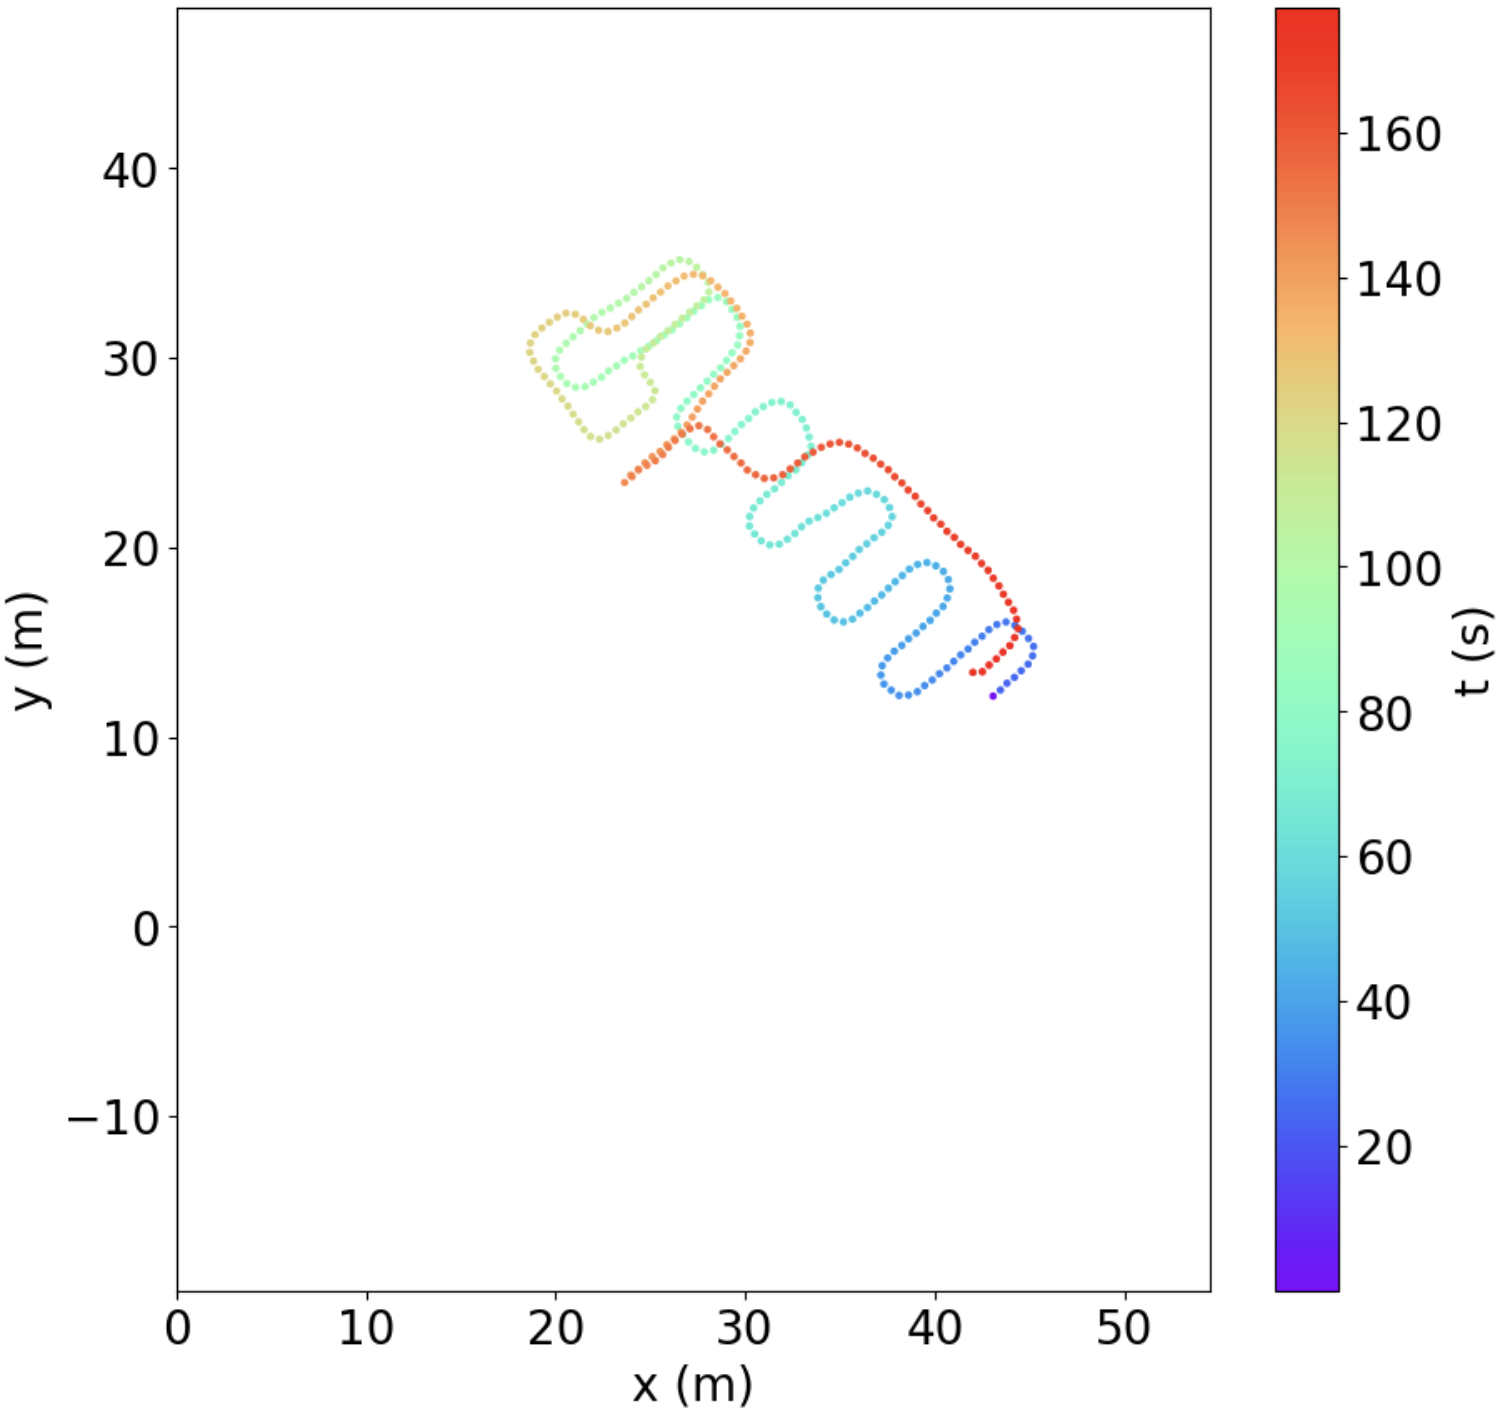
\includegraphics[width=80mm]{image/pdr-remove-drift-two.jpg}
	\caption{ドリフト除去後の軌跡} \label{fig:pdr-remove-drift}
\end{figure}


図\ref{fig:pdr-remove-drift}の軌跡の問題点として初期方向の誤差がある.
初期方向が誤っていると,歩行者の実際の移動経路と大きく異なる軌跡が生成されてしまう.
この問題を解決するために.角度データと環境マップ情報を組み合わせた初期方向の補正アルゴリズムを導入する.
このプロセスは,\_find\_best\_alignment\_angle関数によって実装される.
この関数は,角度データフレーム,地上の真実データ,編集可能なマップ情報,フロア名,およびマップのグリッドサイズを引数として受け取る.
まず,異なる回転角で軌跡の水平垂直方向のカウントを計算し,その後,各回転角度での軌跡が環境マップ上で通行可能かどうかを判断する.
軌跡の水平垂直方向のカウントは,\_calculate\_horizontal\_and\_vertical\_counts関数によって計算される.
この関数は,角度データフレームと回転角を引数として受け取り,回転後の角度に基づいて水平および垂直方向の軌跡カウントを計算する.
軌跡における垂直成分と水平成分を可視化したものが図\ref{fig:color}である.
これにより,回転角度によって軌跡の水平成分と垂直成分の割合の大きさがわかる.
次に,\_calculate\_exist\_counts関数は,回転後の軌跡が環境マップ上で通行可能なポイントの数を計算します.この関数は,角度データフレーム,回転角の結果データフレーム,地上の真実データ,環境マップ情報,フロア名,およびマップのグリッドサイズを引数として受け取る.
最適な方向補正角度は,最も多くの通行可能なポイントを持つ回転角として決定される.
最終的に,\_get\_optimal\_angle関数は,回転後の軌跡が最も多くの通行可能なポイントを持つ回転角度を選択し,これが最適な方向補正角度として選ばれます.この角度を用いて,process\_find\_best\_alignment\_angle関数は,補正された軌跡データを生成する.
この方向補正アルゴリズムを適用することで,PDRに基づく屋内位置推定の精度はさらに向上します.図\ref{fig:pdr-remove-drift}は,方向補正後の軌跡を示しており,補正前の軌跡と比較して,実際の移動経路により密接に一致していることがわかる.

\begin{figure}[h]
	\centering
	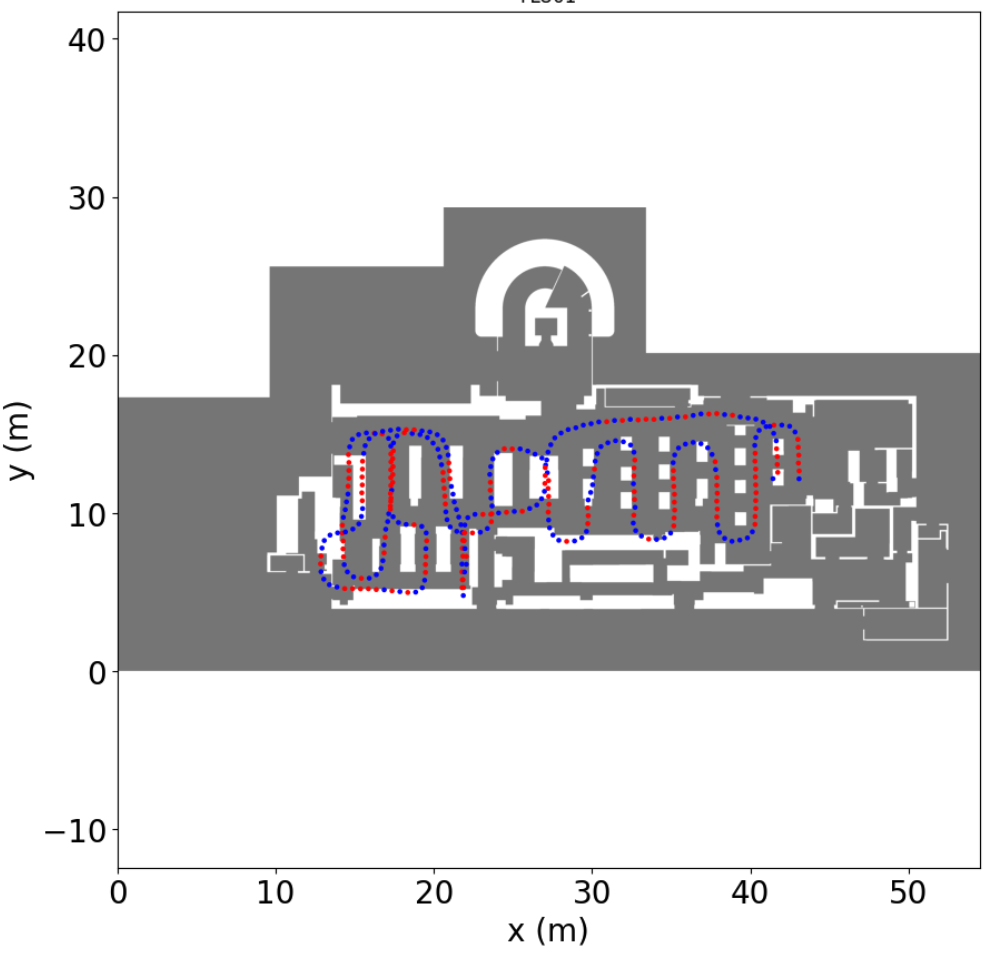
\includegraphics[width=80mm]{image/rb.png}
	\caption{垂直成分と水平成分の可視化}    \label{fig:color}
\end{figure}

\begin{figure}[h]
	\centering
	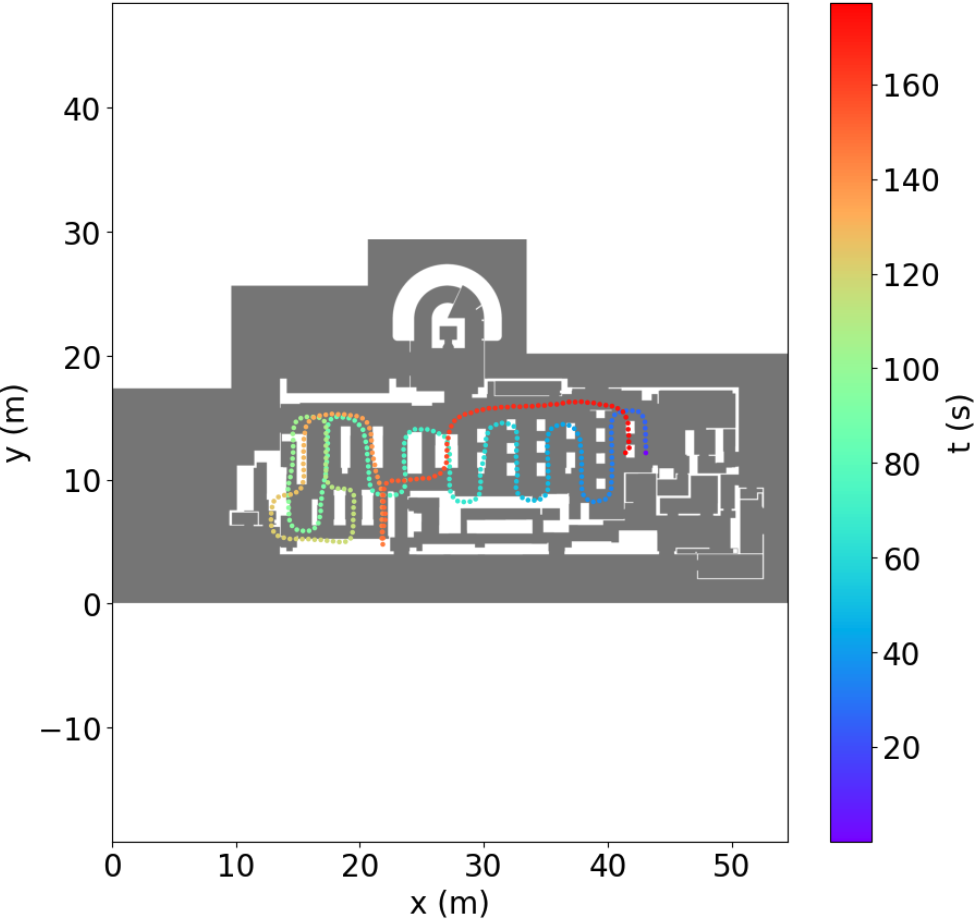
\includegraphics[width=80mm]{image/pdr-rotate.jpg}
	\caption{初期方向の補正後の軌跡}    \label{}
\end{figure}







\bibliography{dicomo}
\bibliographystyle{junsrt}

\end{document}
